% !TeX encoding = UTF-8
% !TeX root = ../main.tex

%% ------------------------------------------------------------------------
%% Copyright (C) 2021,2022 SJTUG
%% 
%% SJTUBeamer Example Document by SJTUG
%% 
%% SJTUBeamer Example Document is licensed under a
%% Creative Commons Attribution-NonCommercial-ShareAlike 4.0 International License.
%% 
%% You should have received a copy of the license along with this
%% work. If not, see <http://creativecommons.org/licenses/by-nc-sa/4.0/>.
%% -----------------------------------------------------------------------

\section{简介}

\subsection{\TeX{} 与 \LaTeX{}}

\begin{frame}[fragile]{\TeX{} 与 \LaTeX{}}
  \begin{columns}[T]
    \column{.8\textwidth}
    \begin{itemize}
      \item \TeX\ (\textipa{/'tEx/},
            \textipa{/'tEk/})
            \begin{itemize}
              \item 最初由 高德纳 (Donald E.~Knuth) 于 1978 年开发的排版系统
              \item 名称源自 technology 的希腊语词根 $\tau\varepsilon\chi$ \par
                    发音接近“泰赫”,而非“泰克斯”
              \item 最新版本为 \TeX\ 3.141592653(2021年1月)
                    \link{https://tex.stackexchange.com/questions/581118/whats-new-in-tex-version-3-141592653}
              \item 漂亮、美观、稳定、通用
              \item 尤其擅长数学公式排版
            \end{itemize}
      \item \LaTeX\ (\textipa{/'la:tEx/}, \textipa{/'leItEk/})
            \begin{itemize}
              \item Leslie Lamport 开发的一种 \TeX{} 格式
              \item 在 \TeX 的基础上提供宏包, 降低使用门槛
              \item 极其丰富的宏包,提供扩展功能
              \item 广泛用于学术界,期刊会议论文模板
              \item 大学学位论文模板,如 \SJTUThesis
            \end{itemize}
    \end{itemize}
    \column{.2\textwidth}
    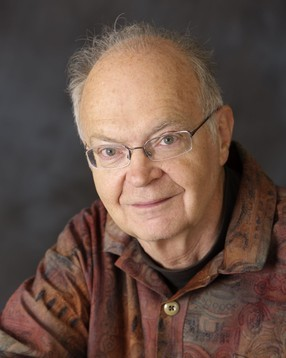
\includegraphics[height=.4\textheight]{Knuth.jpg}

    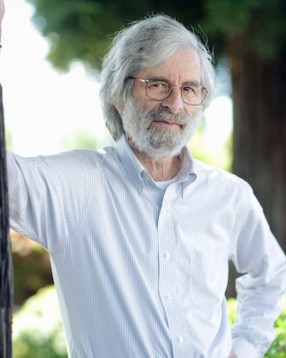
\includegraphics[height=.4\textheight]{Lamport.jpg}
  \end{columns}
\end{frame}

\begin{frame}{和 Word 对比}
  术业有专攻,评价需客观!
  \begin{table}[h]
    \centering
    \begin{tabular}{c|c}
      Microsoft\textsuperscript{\textregistered}  Word & \LaTeX
      \\
      \hline
      字处理工具                                            & 专业排版软件        \\
      容易上手,简单直观                                        & 容易上手          \\
      所见即所得                                            & 所见即所想,所想即所得   \\
      高级功能不易掌握                                         & 进阶难,但一般用不到    \\
      处理长文档需要丰富经验                                      & 和短文档处理基本无异    \\
      花费大量时间调格式                                        & 无需担心格式,专心作者内容 \\
      公式排版差强人意                                         & 尤其擅长公式排版      \\
      二进制格式,兼容性差                                       & 文本文件,易读、稳定    \\
      付费商业许可                                           & 自由免费使用        \\
    \end{tabular}
  \end{table}
\end{frame}

\begin{frame}{\TeX{}排版举例:公式}
  \begin{alertblock}{无编号公式}
    \begin{equation*}
      \mathcal{F}(\xi)=\int_{-\infty}^{\infty} f(x)\mathrm{e}^{-\mathrm{j}2\pi
      \xi x}\,\mathrm{d}x
    \end{equation*}
  \end{alertblock}
  \begin{alertblock}{多行多列公式}
    % Taken from Mathmode.tex
    \begin{align}
      y      & =d                  & z & =1                  \\
      y      & =cx+d               & z & =x+1                \\
      y_{12} & =bx^{2}+cx+d        & z & =x^{2}+x+1\nonumber \\
      y(x)   & =ax^{3}+bx^{2}+cx+d & z & =x^{3}+x^{2}+x+1
    \end{align}
  \end{alertblock}
\end{frame}

\begin{frame}{\TeX{}排版举例:公式}
  \begin{alertblock}{编号多行公式}
    % Taken from Mathmode.tex
    \begin{multline}
      A=\lim_{n\rightarrow\infty}\Delta x\left(a^{2}+\left(a^{2}+2a\Delta
      x+\left(\Delta x\right)^{2}\right)\right.\label{eq:reset}\\
      +\left(a^{2}+2\cdot2a\Delta x+2^{2}\left(\Delta x\right)^{2}\right)\\
      +\left(a^{2}+2\cdot3a\Delta x+3^{2}\left(\Delta x\right)^{2}\right)\\
      +\ldots\\
      \left.+\left(a^{2}+2\cdot(n-1)a\Delta x+(n-1)^{2}\left(\Delta
      x\right)^{2}\right)\right)\\
      =\frac{1}{3}\left(b^{3}-a^{3}\right)
    \end{multline}
  \end{alertblock}
\end{frame}

\begin{frame}{\TeX{}排版举例:图形}
  % https://texample.net/tikz/examples/3d-cone/
  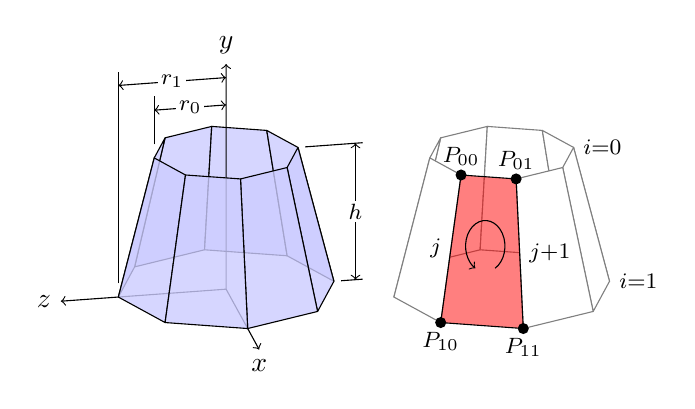
\begin{tikzpicture}[join=round]
    \tikzstyle{conefill} = [fill=blue!20,fill opacity=0.8]
    \tikzstyle{ann} = [fill=white,font=\footnotesize,inner sep=1pt]
    \tikzstyle{ghostfill} = [fill=white]
    \tikzstyle{ghostdraw} = [draw=black!50]
    \filldraw[conefill](-.775,1.922)--(-1.162,.283)--(-.274,.5)
    --(-.183,2.067)--cycle;
    \filldraw[conefill](-.183,2.067)--(-.274,.5)--(.775,.424)
    --(.516,2.016)--cycle;
    \filldraw[conefill](.516,2.016)--(.775,.424)--(1.369,.1)
    --(.913,1.8)--cycle;
    \filldraw[conefill](-.913,1.667)--(-1.369,-.1)--(-1.162,.283)
    --(-.775,1.922)--cycle;
    \draw(1.461,.107)--(1.734,.127);
    \draw[arrows=<->](1.643,1.853)--(1.643,.12);
    \filldraw[conefill](.913,1.8)--(1.369,.1)--(1.162,-.283)
    --(.775,1.545)--cycle;
    \draw[arrows=->,line width=.4pt](.274,-.5)--(0,0)--(0,2.86);
    \draw[arrows=-,line width=.4pt](0,0)--(-1.369,-.1);
    \draw[arrows=->,line width=.4pt](-1.369,-.1)--(-2.1,-.153);
    \filldraw[conefill](-.516,1.45)--(-.775,-.424)--(-1.369,-.1)
    --(-.913,1.667)--cycle;
    \draw(-1.369,.073)--(-1.369,2.76);
    \draw(1.004,1.807)--(1.734,1.86);
    \filldraw[conefill](.775,1.545)--(1.162,-.283)--(.274,-.5)
    --(.183,1.4)--cycle;
    \draw[arrows=<->](0,2.34)--(-.913,2.273);
    \draw(-.913,1.84)--(-.913,2.447);
    \draw[arrows=<->](0,2.687)--(-1.369,2.587);
    \filldraw[conefill](.183,1.4)--(.274,-.5)--(-.775,-.424)
    --(-.516,1.45)--cycle;
    \draw[arrows=<-,line width=.4pt](.42,-.767)--(.274,-.5);
    \node[ann] at (-.456,2.307) {$r_0$};
    \node[ann] at (-.685,2.637) {$r_1$};
    \node[ann] at (1.643,.987) {$h$};
    \path (.42,-.767) node[below] {$x$}
    (0,2.86) node[above] {$y$}
    (-2.1,-.153) node[left] {$z$};
    % Second version of the cone
    \begin{scope}[xshift=3.5cm]
      \filldraw[ghostdraw,ghostfill](-.775,1.922)--(-1.162,.283)--(-.274,.5)
      --(-.183,2.067)--cycle;
      \filldraw[ghostdraw,ghostfill](-.183,2.067)--(-.274,.5)--(.775,.424)
      --(.516,2.016)--cycle;
      \filldraw[ghostdraw,ghostfill](.516,2.016)--(.775,.424)--(1.369,.1)
      --(.913,1.8)--cycle;
      \filldraw[ghostdraw,ghostfill](-.913,1.667)--(-1.369,-.1)--(-1.162,.283)
      --(-.775,1.922)--cycle;
      \filldraw[ghostdraw,ghostfill](.913,1.8)--(1.369,.1)--(1.162,-.283)
      --(.775,1.545)--cycle;
      \filldraw[ghostdraw,ghostfill](-.516,1.45)--(-.775,-.424)--(-1.369,-.1)
      --(-.913,1.667)--cycle;
      \filldraw[ghostdraw,ghostfill](.775,1.545)--(1.162,-.283)--(.274,-.5)
      --(.183,1.4)--cycle;
      \filldraw[fill=red,fill
        opacity=0.5](-.516,1.45)--(-.775,-.424)--(.274,-.5)
      --(.183,1.4)--cycle;
      \fill(-.775,-.424) circle (2pt);
      \fill(.274,-.5) circle (2pt);
      \fill(-.516,1.45) circle (2pt);
      \fill(.183,1.4) circle (2pt);
      \path[font=\footnotesize]
      (.913,1.8) node[right] {$i\hbox{$=$}0$}
      (1.369,.1) node[right] {$i\hbox{$=$}1$};
      \path[font=\footnotesize]
      (-.645,.513) node[left] {$j$}
      (.228,.45) node[right] {$j\hbox{$+$}1$};
      \draw (-.209,.482)+(-60:.25) [yscale=1.3,->] arc(-60:240:.25);
      \fill[black,font=\footnotesize]
      (-.516,1.45) node [above] {$P_{00}$}
      (-.775,-.424) node [below] {$P_{10}$}
      (.183,1.4) node [above] {$P_{01}$}
      (.274,-.5) node [below] {$P_{11}$};
    \end{scope}
  \end{tikzpicture}
  \hspace{1cm}
  % https://texample.net/tikz/examples/line-junctions/
  \tikzstyle{block} = [draw,fill=blue!20,minimum size=2em]
  \def\radius{.7mm}
  \tikzstyle{branch}=[fill,shape=circle,minimum size=3pt,inner sep=0pt]
  \begin{tikzpicture}[>=latex']
    \foreach \y in {1,2,3,4,5} {
        \node at (0,-\y) (input\y) {$i_\y$};
        \node[block] at (2,-\y) (block\y) {$f_\y$};
        \draw[->] (input\y) -- (block\y);
        \draw[->] (block\y.east) -- +(0.5,0);
      }
    \node[block] at (2,-6) (block6) {$f_6$};
    \draw[->] (block6.east) -- +(0.5,0);
    \path (input1) -- coordinate (branch) (block1);
    \tikzstyle{s}=[shift={(0mm,\radius)}]
    \draw[->] (branch) node[branch] {}{ % draw branch junction
      \foreach \c in {2,3,4,5} {
          [shift only] -- ([s]input\c -| branch) arc(90:-90:\radius)
        }
    } |- (block6);
  \end{tikzpicture}
\end{frame}

\begin{frame}{\TeX{}排版举例:文档}
  \begin{columns}
    \begin{column}{.45\textwidth}
      \begin{figure}[h]
        \centering
        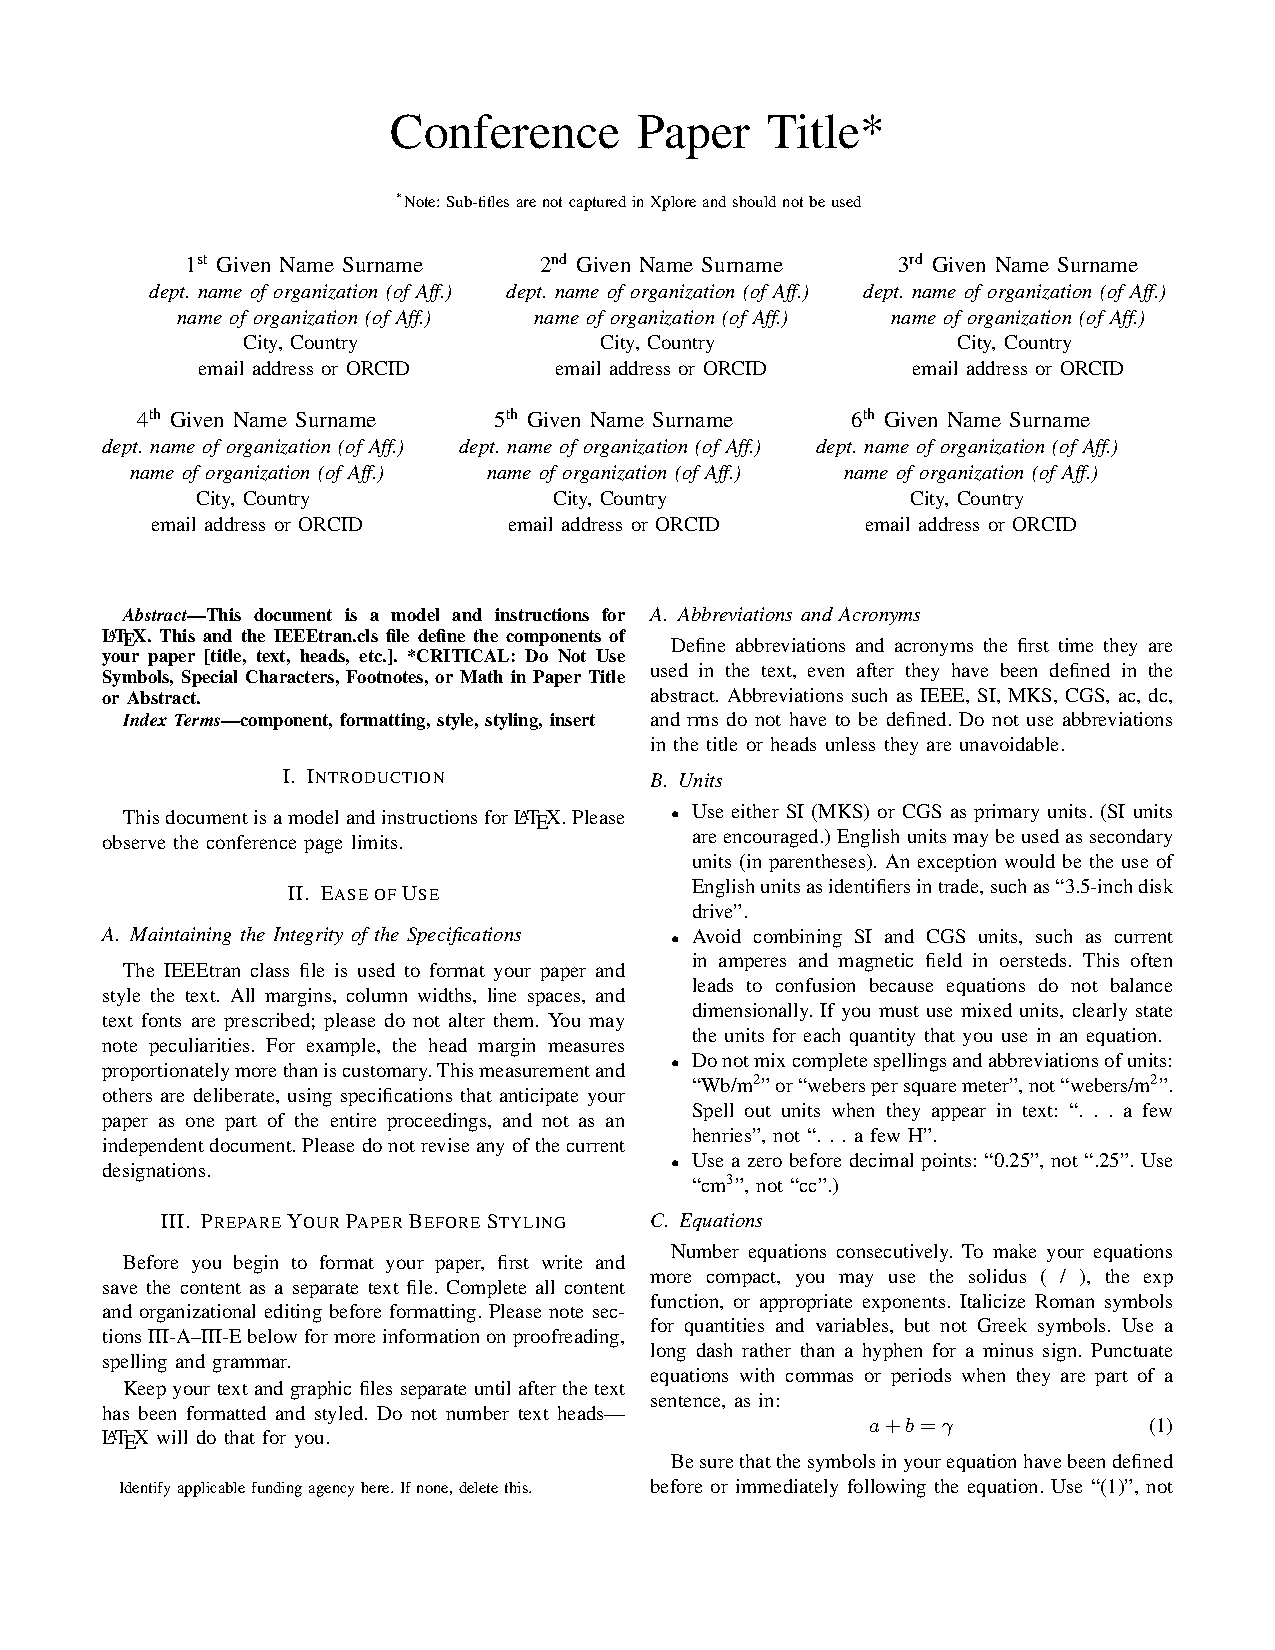
\includegraphics[width=.8\textwidth]{ieee-conference-template.pdf}
      \end{figure}
    \end{column}
    \begin{column}{.45\textwidth}
      \color{red}
      \heartpar{\footnotesize%
        Lorem ipsum dolor sit amet, consectetur adipisicing elit, sed do
        eiusmod
        tempor incididunt ut labore et	dolore magna aliqua. Ut enim ad minim
        veniam, quis nostrud exercitation ullamco laboris nisi ut aliquip ex ea
        commodo consequat. Duis aute irure dolor in reprehenderit in voluptate
        velit esse cillum dolore eu fugiat nulla pariatur. Excepteur sint
        occaecat cupidatat non proident, sunt in culpa qui officia deserunt
        mollit anim id est laborum.}
    \end{column}
  \end{columns}
\end{frame}

\begin{frame}{\TeX{}排版举例:幻灯片}
  \begin{columns}
    \begin{column}{.45\textwidth}
      \begin{figure}[h]
        \centering
        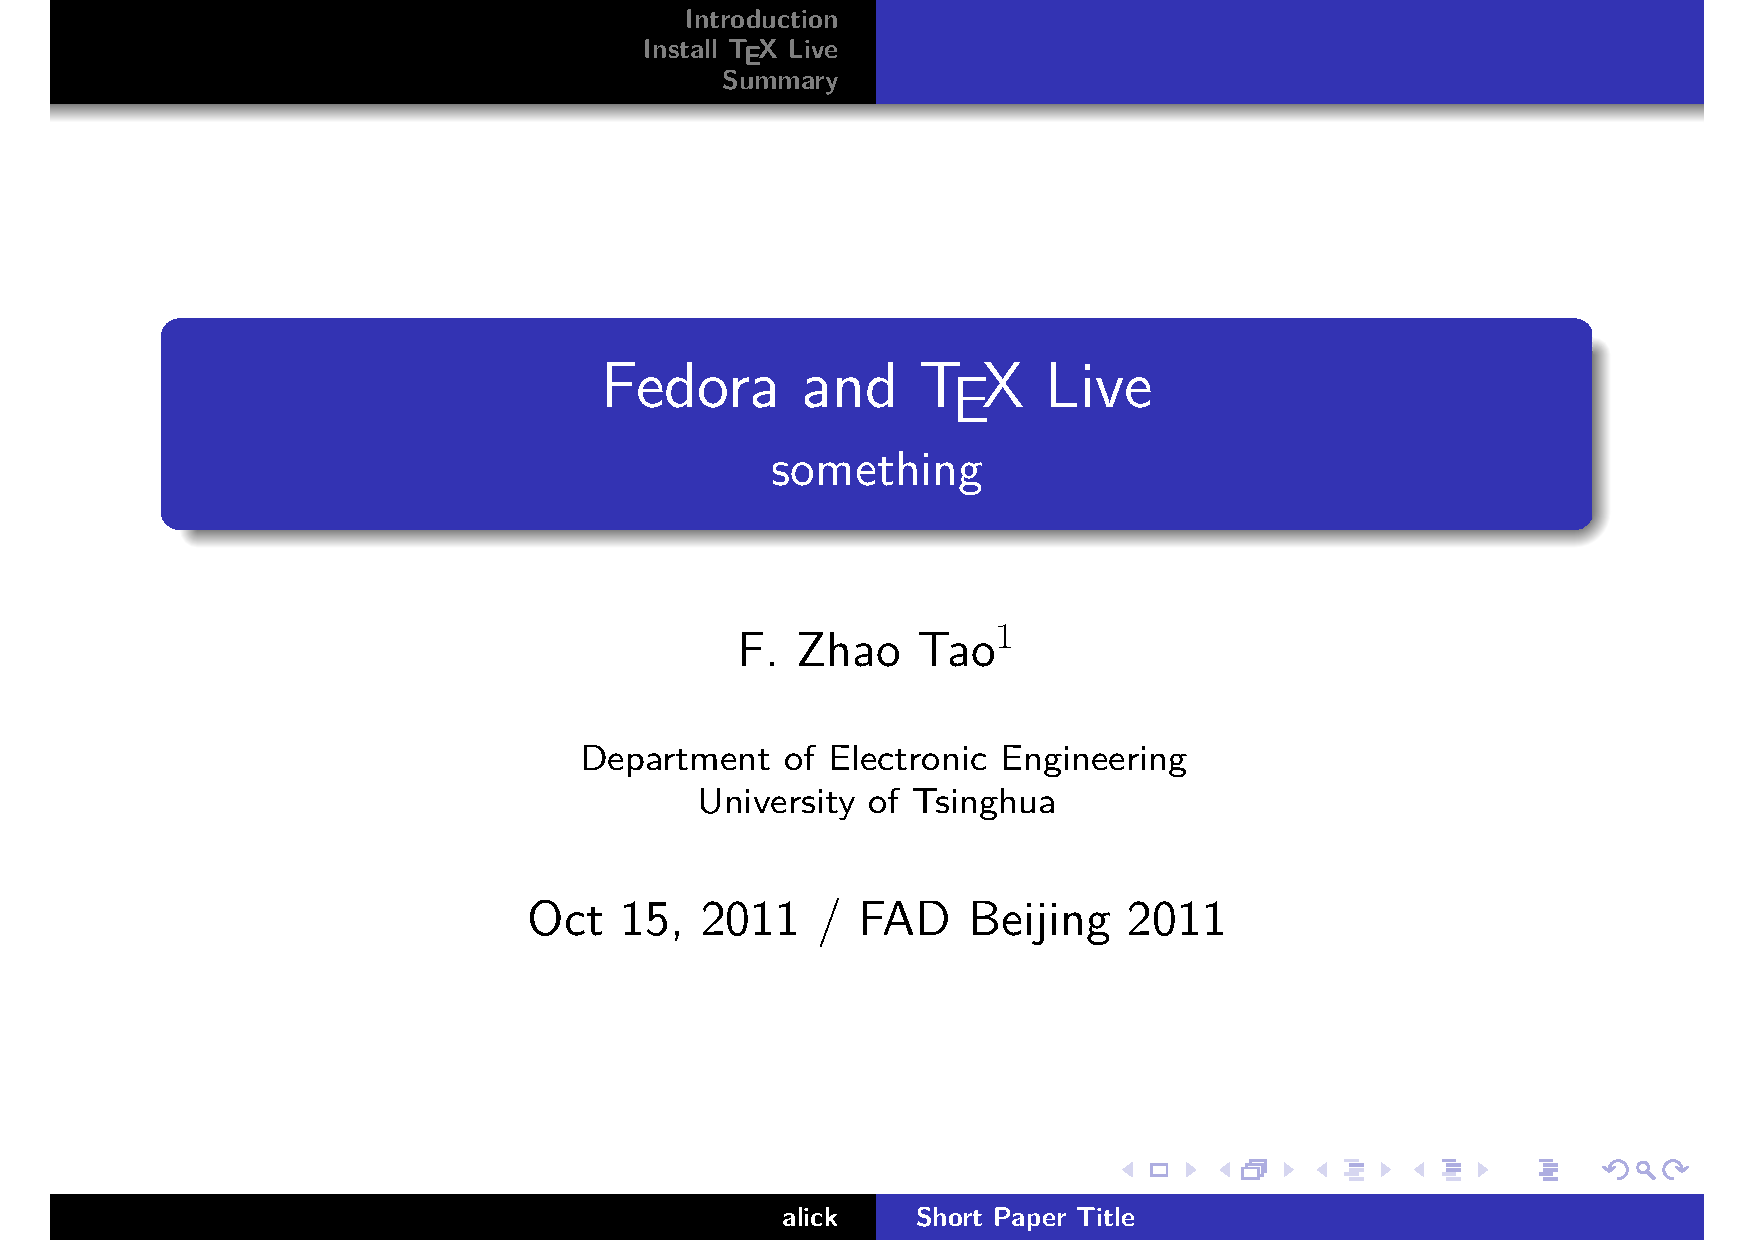
\includegraphics[width=\textwidth]{slides-beamer.pdf}
      \end{figure}
    \end{column}
    \begin{column}{.45\textwidth}
      \begin{figure}[h]
        \centering
        % https://www.overleaf.com/latex/templates/zut-fibeamer/ksnwzmnhktvn
        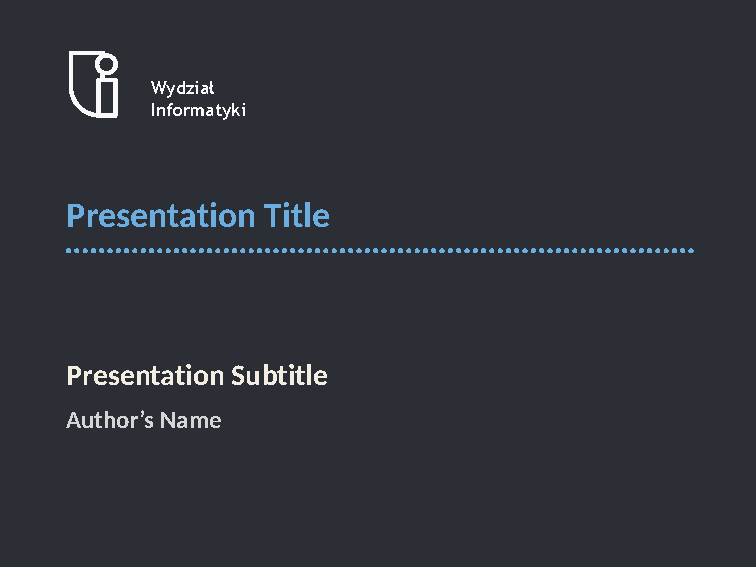
\includegraphics[width=\textwidth]{zut-fibeamer.pdf}
      \end{figure}
    \end{column}
  \end{columns}
\end{frame}

\subsection{安装}

\begin{frame}{如何安装 \hologo{(La)TeX}?}
  \begin{itemize}
    \item \TeX{}发行版(Distro)
          \begin{itemize}
            \item 引擎、宏包、字体、文档的综合体
            \item 常见\TeX{}发行版:
                  \alert{\TL}, \MacTeX, \MiKTeX, \CTeX
          \end{itemize}
    \item \TL
          \begin{itemize}
            \item 跨平台:Windows, Linux, macOS (\MacTeX{} $\approx$ \TL)
            \item 每年四月左右发布以年份命名的新版本,当前为 \TL 2021
            \item 官方维护,入门首选
          \end{itemize}
    \item \MiKTeX
          \begin{itemize}
            \item 最早专为 Windows 开发,现亦有 Linux 和 macOS 版本
            \item 宏包随用随装
            \item Christian Schenk 个人维护(是个狠人)
          \end{itemize}
    \item \CTeX
          \begin{itemize}
            \item 中科院吴凌云研究员基于 \MiKTeX 开发
            \item 极大的方便了中文 \TeX 用户
            \item 2012 年之后停止开发,\alert{不再建议}使用
          \end{itemize}
  \end{itemize}
\end{frame}

\begin{frame}[fragile]
  \frametitle{下载}
  \begin{itemize}
    \item 注意!
          \begin{itemize}
            \item 新手建议安装完整版 \TL (\MacTeX)
            \item 建议使用 ISO 镜像离线安装
            \item 在线安装要求网络稳定
            \item Windows 下不要放在带有中文的路径中
          \end{itemize}
    \item 选择国内 CTAN 镜像
          \begin{itemize}
            \item 上海交通大学 Linux 用户组 软件源镜像服务
                  \link{https://mirrors.sjtug.sjtu.edu.cn/}
            \item {\footnotesize
                  \url{https://mirrors.sjtug.sjtu.edu.cn/ctan/systems/texlive/Images/texlive.iso}
                  }
            \item 更多镜像 \link{http://mirror.ctan.org/README.mirrors}
          \end{itemize}
    \item 可选步骤:校验安装包
          \begin{itemize}
            \item \verb|Get-FileHash -Algorithm SHA512 texlive.iso|
            \item \verb|sha512sum --check texlive.iso.sha512|
          \end{itemize}
  \end{itemize}
\end{frame}

\begin{frame}[fragile]
  \frametitle{安装}
  \begin{itemize}
    \item Windows
          \begin{itemize}
            \item 挂载或解压下载的 ISO,运行 \verb|install-tl-windows.bat|
            \item 切换默认仓库为国内镜像(如 SJTUG)可加速今后升级
          \end{itemize}
    \item macOS
          \begin{itemize}
            \item 推荐使用独立的 pkg 安装包
                  \link{https://mirrors.sjtug.sjtu.edu.cn/ctan/systems/mac/mactex/MacTeX.pkg}
            \item 也可以使用 \TL 安装包安装
                  \link{http://www.tug.org/mactex/mactex-unix-download.html}
            \item 可选:Homebrew \link{https://brew.sh/}
          \end{itemize}
    \item Linux
          \begin{itemize}
            \item 不推荐从 Linux 发行版仓库直接安装(更新缓慢)
            \item 图形安装界面需要 Perl Tk 模块
                  \begin{lstlisting}[language=bash]
sudo apt-get install perl-tk
sudo ./install-tl -gui=perltk
        \end{lstlisting}
          \end{itemize}
  \end{itemize}
\end{frame}

\begin{frame}[fragile]
  \frametitle{安装(续)}
  \begin{itemize}
    \item Linux
          \begin{itemize}
            \item 添加环境变量到 \nolinkurl{~/.bashrc} 文件:
                  \begin{lstlisting}[language=bash]
export PATH=/usr/local/texlive/2021/bin/x86_64-linux:$PATH
export MANPATH=/usr/local/texlive/2021/texmf/doc/man:$MANPATH
export INFOPATH=/usr/local/texlive/2021/texmf/doc/info:$INFOPATH
          \end{lstlisting}
            \item 安装一个 dummy package,让系统的包管理器知道 \TL 已经装过了
                  \begin{itemize}
                    \item Debian/Ubuntu 用户参照手册做一个包即可
                          \link{https://www.tug.org/texlive/debian.html\#vanilla}
                    \item Arch Linux 用户装 AUR 里的 \verb|texlive-dummy|
                    \item Feodra 用户可以直接下载
                          \link{https://copr.fedoraproject.org/coprs/fatka/texlive-dummy/}
                  \end{itemize}
          \end{itemize}
    \item 安装指南
          \begin{itemize}
            \item 《一份简短的关于 \LaTeX{} 安装的介绍》
                  \link{https://mirrors.sjtug.sjtu.edu.cn/ctan/info/install-latex-guide-zh-cn/install-latex-guide-zh-cn.pdf}
            \item 《\TL{} 指南中文版》
                  \link{https://www.tug.org/texlive/doc/texlive-zh-cn/texlive-zh-cn.pdf}
            \item 更多参考:
                  \link{http://zhuanlan.zhihu.com/LaTeX/20069414}
                  \link{https://stone-zeng.github.io/2018-05-13-install-texlive-ubuntu/}
          \end{itemize}
  \end{itemize}
\end{frame}

\begin{frame}{选择编辑器}
  \begin{itemize}
    \item 专用编辑器
          \begin{itemize}
            \item TeXworks、TeXShop、\alert{TeXStudio}、TeXmaker、WinEdt 等
          \end{itemize}
    \item 通用编辑器(安装 \LaTeX{} 插件)
          \begin{itemize}
            \item Vim、Emacs、\alert{VS Code}、Sublime、Atom 等
          \end{itemize}
    \item 在线协作平台
          \begin{itemize}
            \item OverLeaf \link{https://www.overleaf.com/}, \sout{ShareLaTeX}(已经与前者合并)
            \item 交大 LaTeX 文档助手 \link{https://latex.sjtu.edu.cn/}(基于 OverLeaf)
          \end{itemize}
    \item 编辑器对比:\link{https://tex.stackexchange.com/q/339}
          \link{https://en.wikipedia.org/wiki/Comparison_of_TeX_editors}
          \link{https://www.zhihu.com/question/19954023}
  \end{itemize}
\end{frame}

\begin{frame}[fragile]{安装或更新宏包}
  \begin{itemize}
    \item 有时需要自己安装宏包
          \begin{itemize}
            \item 发行版没有预装
            \item 宏包需要更新
          \end{itemize}
    \item \TL
          \begin{itemize}
            \item 设置仓库地址 \verb|tlmgr option repository| {\footnotesize\ttfamily
                  https://mirrors.sjtug.sjtu.edu.cn/CTAN/systems/texlive/tlnet}
            \item \verb|tlmgr install <pkgname>| 安装、 \verb|tlmgr update --self --all| 全部更新
            \item \faWindows{} 开始菜单里找 TeX Live Manager
          \end{itemize}
    \item \MiKTeX
          \begin{itemize}
            \item \faWindows{} 开始菜单里找 MiKTeX Console
          \end{itemize}
  \end{itemize}
\end{frame}
